% sections/01_architecture.tex
\section{Server Architecture}
\label{sec:server}

The EC2 game server is a single-threaded \texttt{asyncio} reactor
whose processing is decomposed into four stages (T1--T4)
(Figure~\ref{fig:pipeline}) connected by lock-free queues, inspired
by the staged event-driven topology of SEDA~\cite{seda}.
Unlike classical SEDA, there are no thread pools: the hot path is
I/O-bound with negligible CPU work per tick, so threading would add lock contention and
context-switch overhead for no throughput gain. T1--T3 therefore run
as cooperative coroutines on one OS thread; only T4 (blocking Redis
writes) requires a second thread. This gives the structural benefits
of staged decomposition (per-stage observability, backpressure
isolation, independent testability) without shared-state locking.

\textbf{T1} (\texttt{DatagramProtocol} callback) enqueues each UDP datagram on \texttt{packet\_queue}.

\textbf{T2} (game tick) drains the queue each tick, runs authoritative game logic, builds the outbound \texttt{PKT\_GAME\_STATE}, and pushes it to \texttt{broadcast\_queue} (T3) and \texttt{write\_queue} (T4). A monotonic self-correcting scheduler compensates for event-loop drift.

\textbf{T3} awaits \texttt{broadcast\_queue} and calls \texttt{transport.sendto()} for each node.

\textbf{T4} blocks on \texttt{write\_queue.get()}, batches all \texttt{HSET} operations into a single Redis pipeline per tick.

\begin{figure}[h]
  \centering
  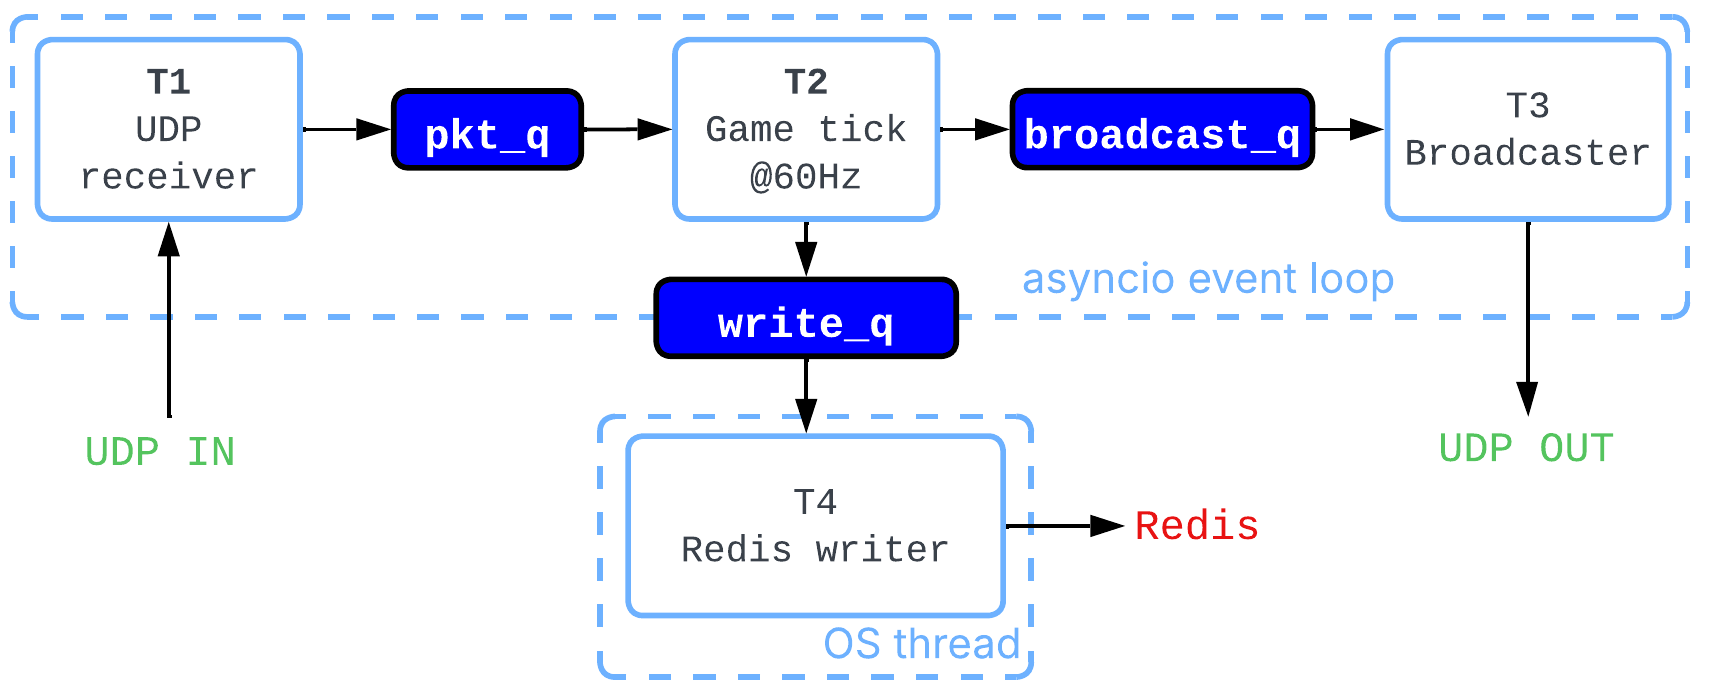
\includegraphics[width=\columnwidth]{images/event_loop.png}
  \caption{The Server Reactor pipeline with SEDA-inspired topology.}
  \label{fig:pipeline}
\end{figure}

\paragraph{Authority model:}
Nodes are authoritative for position; the server is authoritative for all match events. Sequence validation drops stale/replayed packets via 16-bit circular comparison. Wall-collision clamping snaps illegal positions using axis-aligned slide with binary-search fallback. Ghost AI scores 10 candidate headings per tick by proximity progress and steer-change penalty: at $n{=}4$ entities the $O(n^2)$ proximity loop is negligible.
